
\subsection{Información Búsqueda}
\begin{itemize}
	\item Secuencia original: \texttt{CRISTIANMAREIRA}
	\item Alineamiento significativo:
	\begin{itemize}
		\item Descripción: DfpF [Agrobacterium tumefaciens]
		\item Puntuación máxima: $31.6$ bits (67)
		\item Puntuación total: $31.6$ 
		\item Query coverage: $93\%$
		\item Valor de E: $12$
	\end{itemize}
\end{itemize}


\subsection{Dotplot}
%    * Muestre el dotplot entre su nombre
%		(en la forma que se usó en la búsqueda)
%		y un segmento de la proteína encontrada,
%		que incluya el match pero sea más largo
%		que el query (digamos, 3 veces la longitud).
\begin{tiny}
\begin{tabular}{|p{0.0025cm}|p{0.0025cm}|p{0.0025cm}|p{0.0025cm}|p{0.0025cm}|p{0.0025cm}|p{0.0025cm}|p{0.0025cm}|p{0.0025cm}|p{0.0025cm}|p{0.0025cm}|p{0.0025cm}|p{0.0025cm}|p{0.0025cm}|p{0.0025cm}|p{0.0025cm}|p{0.0025cm}|p{0.0025cm}|p{0.0025cm}|p{0.0025cm}|p{0.0025cm}|p{0.0025cm}|p{0.0025cm}|p{0.0025cm}|p{0.0025cm}|p{0.0025cm}|p{0.0025cm}|p{0.0025cm}|p{0.0025cm}|p{0.0025cm}|p{0.0025cm}|p{0.0025cm}|p{0.0025cm}|p{0.0025cm}|p{0.0025cm}|p{0.0025cm}|p{0.0025cm}|p{0.0025cm}|p{0.0025cm}|p{0.0025cm}|}
\hline
  & g & r & s & v & e & d & t & a & w & g & i & i & r & i & a & v & a & n & m & a & r & a & i & r & a & v & a & m & d & k & g & h & d & l & k & s & f & a & m\\\hline
c &   &   &   &   &   &   &   &   &   &   &   &   &   &   &   &   &   &   &   &   &   &   &   &   &   &   &   &   &   &   &   &   &   &   &   &   &   &   &   \\\hline
r &   & * &   &   &   &   &   &   &   &   &   &   & * &   &   &   &   &   &   &   & * &   &   & * &   &   &   &   &   &   &   &   &   &   &   &   &   &   &   \\\hline
i &   &   &   &   &   &   &   &   &   &   & * & * &   & * &   &   &   &   &   &   &   &   & * &   &   &   &   &   &   &   &   &   &   &   &   &   &   &   &   \\\hline
s &   &   & * &   &   &   &   &   &   &   &   &   &   &   &   &   &   &   &   &   &   &   &   &   &   &   &   &   &   &   &   &   &   &   &   & * &   &   &   \\\hline
t &   &   &   &   &   &   & * &   &   &   &   &   &   &   &   &   &   &   &   &   &   &   &   &   &   &   &   &   &   &   &   &   &   &   &   &   &   &   &   \\\hline
i &   &   &   &   &   &   &   &   &   &   & * & * &   & * &   &   &   &   &   &   &   &   & * &   &   &   &   &   &   &   &   &   &   &   &   &   &   &   &   \\\hline
a &   &   &   &   &   &   &   & * &   &   &   &   &   &   & * &   & * &   &   & * &   & * &   &   & * &   & * &   &   &   &   &   &   &   &   &   &   & * &   \\\hline
n &   &   &   &   &   &   &   &   &   &   &   &   &   &   &   &   &   & * &   &   &   &   &   &   &   &   &   &   &   &   &   &   &   &   &   &   &   &   &   \\\hline
m &   &   &   &   &   &   &   &   &   &   &   &   &   &   &   &   &   &   & * &   &   &   &   &   &   &   &   & * &   &   &   &   &   &   &   &   &   &   & * \\\hline
a &   &   &   &   &   &   &   & * &   &   &   &   &   &   & * &   & * &   &   & * &   & * &   &   & * &   & * &   &   &   &   &   &   &   &   &   &   & * &   \\\hline
r &   & * &   &   &   &   &   &   &   &   &   &   & * &   &   &   &   &   &   &   & * &   &   & * &   &   &   &   &   &   &   &   &   &   &   &   &   &   &   \\\hline
e &   &   &   &   & * &   &   &   &   &   &   &   &   &   &   &   &   &   &   &   &   &   &   &   &   &   &   &   &   &   &   &   &   &   &   &   &   &   &   \\\hline
i &   &   &   &   &   &   &   &   &   &   & * & * &   & * &   &   &   &   &   &   &   &   & * &   &   &   &   &   &   &   &   &   &   &   &   &   &   &   &   \\\hline
r &   & * &   &   &   &   &   &   &   &   &   &   & * &   &   &   &   &   &   &   & * &   &   & * &   &   &   &   &   &   &   &   &   &   &   &   &   &   &   \\\hline
a &   &   &   &   &   &   &   & * &   &   &   &   &   &   & * &   & * &   &   & * &   & * &   &   & * &   & * &   &   &   &   &   &   &   &   &   &   & * &   \\\hline
\end{tabular}
\end{tiny}

Dotplot generado por un script en python realizado para la tarea, se encuentra en el anexo~\ref{sec:anexo}.

\subsection{Alineamiento}
%    * Muestre el alineamiento entre su nombre
%		y el segmento de la proteína.
El query inicial fue \texttt{CRISTIANMAREIRA}
pero no se encontró ningún match exacto,
por lo tanto sólo se encontró una aproximación a
partir del query 2 con el siguiente texto \texttt{RIA-VANMARAIRA},
por lo tanto algunos datos:
\begin{itemize}
	\item Puntaje 31.6 bits (67)
	\item Esperado = 12
	\item Igualdades = 10/14 (72\%)
	\item Positivos = 11/14 (79\%)
	\item Gaps = 1/14 (7\%)
\end{itemize}

Secuencias del query y del match:

\begin{tabular}{lcl}
Query  2   & RISTIANMAREIRA & 15\\
           & RI\ \ \ \ +ANMAR\ IRA & \\
Sbjct  443 & RIA-VANMARAIRA & 455\\
\end{tabular}

\subsection{Información de la proteína}
%    * ¿Qué función cumple la proteína?
%		¿Se sabe con certeza (base experimental), o es una hipótesis?
%		¿Se conoce su estructura 3D?
La proteína \textbf{DfpF} de la \emph{Agrobacterium tumefaciens} no
posee información acerca de su función en la página de ``GenBank''~\cite{match1}, pero investigando, pude dar con otro sitio llamado ``UnitPro''~\footnote{\url{http://www.uniprot.org/}},
en el cual pude encontrar la proteína~\footnote{\url{http://www.uniprot.org/uniprot/Q9ADX5}}
y conocer un poco de información acerca de su función, que se explica a continuación:

\begin{itemize}
	\item Actividad Hidrolasa (Hydrolase Activity):
	\begin{itemize}
		\item Catálisis de la hidrólisis de varios enlaces, por ejemplo, C-O, C-N, C-C,
			también de enlaces de anhídrido fosfórico, etc.
		\item La hidrolasa es el nombre sistemático para cualquier enzima de clase
			EC 3~\footnote{Los números EC (Enzyme Commission numbers) son un esquema de clasificación
			numérica para las enzimas, basado en las reacciones químicas que catalizan.}.
	\end{itemize}
\end{itemize}

Algunos conceptos claves:
\begin{itemize}
	\item \emph{Hidrolasa:}
		Una hidrolasa es una enzima capaz de hidrolizar un enlace químico.
	\item \emph{Enzima:}
		Las enzimas son moléculas de naturaleza proteica que catalizan
		reacciones químicas, siempre que sea termodinámicamente posible.
	\item \emph{Hidrolizar:}
		Es una reacción química entre agua y otra sustancia.
	\item \emph{Enlace químico:}
		Un enlace químico es el proceso físico responsable de las interacciones atractivas entre átomos y moléculas, y que confiere estabilidad a los compuestos químicos diatómicos y poliatómicos
	\item \emph{Catálisis:}
		La catálisis es el proceso por el cual se aumenta o disminuye la velocidad de una reacción química.
\end{itemize}

Sobre la veracidad de su función, podríamos decir que es cierta,
debido a que en la referencia anterior de ``UnitProt'' nos señala
que con respecto a algunos atributos de la proteína son:
\begin{itemize}
	\item Largo de la secuencia: 706 AA.
	\item Estado de la secuencia: Completo.
	\item Existencia de la proteína: Predicho.
\end{itemize}

Por lo que al conocer la secuencia completa, se infiere la veracidad
del establecimiento de su función.

Al buscar un modelo en 3d, no se encontró ninguno,
y el más parecido fue uno a partir de un template ``3cetA''~\footnote{\url{http://www.proteinmodelportal.org/?pid=modelDetail&pmpuid=1000009972743&range_from=1&range_to=706&ac=&zid=async}},
el cual tenía un $14\%$ de igualdad con la proteína estudiada (DfpF).

        \begin{figure}[!h]
            \begin{center}
                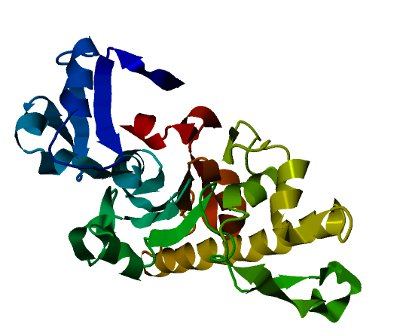
\includegraphics[width=0.3\textwidth]{img/parecida}
            \end{center}
            \caption{Modelo basado en el template 3cetA con un 14\% de igualdad con la proteína DfpF}
        \end{figure}

\subsection{Organismo}
%    * El organismo en que la encontró: ¿qué es?
%		(clasificación, descripción, imagen si existe)
\begin{itemize}
	\item \textbf{Nombre:}
		 Agrobacterium tumefaciens (Smith \& Townsend, 1907) Conn, 1942)
	\begin{itemize}
		\item Clasificación científica:
		\begin{itemize}
			\item Dominio: 	Bacteria
			\item Filo: 	Proteobacteria
			\item Clase: 	Proteobacteria alfa
			\item Orden: 	Rhizobiales
			\item Familia: 	Rhizobiaceae
			\item Género: 	Agrobacterium
			\item Especie: 	A. tumefaciens
		\end{itemize}
	\end{itemize}
	\item \textbf{Descripción:}
		Es una bacteria que produce en ciertas plantas dicotiledóneas unas especies
		de tumores conocidos como ``agallas'' o también ``tumores del cuello'',
		los cuales crecen en la zona en la que se une la raíz y el tallo de la planta.

		Este organismo es una proteobacteria alpha perteneciente a la familia de ``Rhizobiaceae'',
		la que incluye también a las fijadoras de nitrógeno que viven en el proceso de simbiosis
		de ciertas legumbres, pero la Agrobacterium se diferencia por ser un parásito y causa
		mucho daño a la planta que afecta.

		Es importante recalcar que nuestro organismo estudiado no es el único ni más común
		causante de estos tipos de tumores en las plantas, ya que muchos otros son causados
		por algunos tipos de larvas e insectos, los que van agregando sustancias que les
		van produciendo los tumores.
		
		\begin{itemize}
			\item  Método de infección:

				La guía que utiliza ésta bacteria son ciertas sustancias que va excretando la planta,
				proveniente de pequeñas heridas, por las cuales ingresa al organismo. Una vez dentro,
				se va ubicando en ciertos espacios intercelulares donde va transfiriendo a las células
				de la planta un fragmento de su material genético, que es un plásmido~\footnote{ADN circular extracromosómico bacteriano}
				para transferir un segmento de ADN conocido como T-DNA, que se integra en una zona del
				genoma de la planta.			

				El T-DNA que se inserta por la Agrobacterium contiene genes que van provocando la producción de
				ciertos regulares del crecimiento vegetal, de los cuales van resultando los tumores.
				El T-DNA también contiene ciertos genes codificadores de enzimas que van causando que la planta
				produzca aminoácidos especializados llamados opinas, los cuales son fuente de energía
				específica para la Agrobacterium, pero no para otros organismos, lo que crea el ambiente
				ideal para que se pueda desarrollar sin ningún problema.

			\item Biotecnología:

				Un aspecto muy importante de la Agrobacterium es que su capacidad de trasmisión de ADN
				está siendo extensamente explotada en biotecnología, ya que se utiliza su medio de inserción
				de genes foráneos dentro de las plantas y desarrollar ciertos organismos modificados
				genéticamente. Entonces la idea es tratar de utilizarlo como un vehículo óptimo para
				ciertas operaciones de ingeniería genética. Entre los organismos transgénicos creados por
				este método están las plantas productoras del insecticida Bt, una toxina originalmente 
				producida por el \emph{Bacillus thuringiensis}.

				Los laboratorios del proyecto australiano CAMBIA obtuvieron relevancia al desarrollar una versión
				de Agrobacterium tumefaciens modificada mediante tecnología de código abierto.

	\end{itemize}

	\item \textbf{Imagen:}

		Se muestra una foto del organismo en~\ref{fig:1} y una de la acción de inserción en células de zanahoria~\ref{fig:2}.
		\begin{figure}[!h]
			\begin{center}
				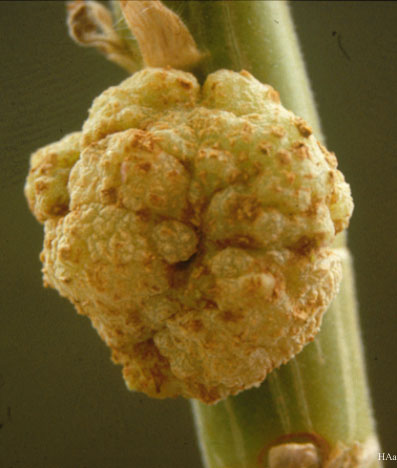
\includegraphics[width=0.3\textwidth]{img/bacteria}
			\end{center}
			\caption{Agrobacterium tumefaciens}
			\label{fig:1}
		\end{figure}

		\begin{figure}[!h]
			\begin{center}
				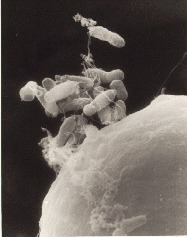
\includegraphics[width=0.3\textwidth]{img/bacteria2}
			\end{center}
			\caption{A. tumefaciens adheriendose a células de zanahoria}
			\label{fig:2}
		\end{figure}
		
\end{itemize}

\subsection{Codificación}
%    * ¿Dónde y cómo está codificada la proteína?
%		(Indique la ubicación de la CDS -"coding sequence" - de DNA que codifica la proteína, y acaso está en
%		la hebra primaria o secundaria, si es continua o tiene interrupciones, etc.; incluya el código de acceso o URL
%		de la secuencia de DNA)

Según la información entregada por ``GenBank'',
La información acerca del CDS es la siguiente:
\begin{verbatim}
 CDS        1..706
            /gene="dfpF"
            /coded_by="complement(AF065242.2:35676..37796)"
            /transl_table=11
\end{verbatim}

Por lo que más adelante podemos ver la secuencia continua con los 706 aminoácidos:

\begin{verbatim}
ORIGIN      
        1 mfldrgherq gsgmkprpqr kdqsimgnir vgidvggtft dftvlddetg gmrhfkvsst
       61 phdpseaiei gitgfgkrgl qssdvvhfgh gttvatnmvi errggktgll ttegfrdvle
      121 igrqtrpdlf dmsvrkpdpl vvrplrleva erlgpagevi vplddagvea aakrfkeegv
      181 eavaigflhs yrnpaheqra aeiirqhlpd vfislssdvl pefreyeris ttvmnaylmp
      241 rmdgylerfm arsrkagvka kpytihsngg lmstetarny pvrtclsgpa agvvgaslvg
      301 kaasfpniit ydvggtstdv aliangkpay stdrdvagys ircpmvdvhv igagggsiaw
      361 lddagglkvg pqsaaavpgp aaygkggtda tisdanivlq rlnpvalldg ampvdreaal
      421 raigavatqi grsvedtawg iiriavanma rairavamdk ghdlksfalm afggagplhs
      481 slvaaetglk tviipespgt mcargvllsd vtrdfvstqi kwaqgeawld iasalqglel
      541 qakewleaet ipdekralqh iaearyagqn heirvegils taedfttrfa eahrvvygya
      601 lenhpveivn lrvqaighag rplqtvdgaa gsmkdaivge revyidpqag wqtvpvykrp
      661 ampqgetftg paiveeltst tyilpgqsgv vdaygniils fvkdra
\end{verbatim}

Pero como es necesario saber la secuencia de ADN,
en la información del CDA se señala un link~\footnote{\url{http://www.ncbi.nlm.nih.gov/nuccore/12831440?from=35676&to=37796&report=gbwithparts}}
en donde nos señala la secuencia de ADN donde la proteína fue codificada:

\begin{verbatim}
CDS   complement(1..2121)
           /gene="dfpF"
           /codon_start=1
           /transl_table=11
           /product="DfpF"
           /protein_id="AAK08622.1"
           /db_xref="GI:12831467"
           /translation="MFLDRGHERQGSGMKPRPQRKDQSIMGNIRVGIDVGGTFTDFTV
           LDDETGGMRHFKVSSTPHDPSEAIEIGITGFGKRGLQSSDVVHFGHGTTVATNMVIER
           RGGKTGLLTTEGFRDVLEIGRQTRPDLFDMSVRKPDPLVVRPLRLEVAERLGPAGEVI
           VPLDDAGVEAAAKRFKEEGVEAVAIGFLHSYRNPAHEQRAAEIIRQHLPDVFISLSSD
           VLPEFREYERISTTVMNAYLMPRMDGYLERFMARSRKAGVKAKPYTIHSNGGLMSTET
           ARNYPVRTCLSGPAAGVVGASLVGKAASFPNIITYDVGGTSTDVALIANGKPAYSTDR
           DVAGYSIRCPMVDVHVIGAGGGSIAWLDDAGGLKVGPQSAAAVPGPAAYGKGGTDATI
           SDANIVLQRLNPVALLDGAMPVDREAALRAIGAVATQIGRSVEDTAWGIIRIAVANMA
           RAIRAVAMDKGHDLKSFALMAFGGAGPLHSSLVAAETGLKTVIIPESPGTMCARGVLL
           SDVTRDFVSTQIKWAQGEAWLDIASALQGLELQAKEWLEAETIPDEKRALQHIAEARY
           AGQNHEIRVEGILSTAEDFTTRFAEAHRVVYGYALENHPVEIVNLRVQAIGHAGRPLQ
           TVDGAAGSMKDAIVGEREVYIDPQAGWQTVPVYKRPAMPQGETFTGPAIVEELTSTTY
           ILPGQSGVVDAYGNIILSFVKDRA"
\end{verbatim}

La tabla de traducción utilizada en el proceso de codificación es la número 11 de las bases
de datos de ``GenBank'':

\begin{verbatim}
    AAs  = FFLLSSSSYY**CC*WLLLLPPPPHHQQRRRRIIIMTTTTNNKKSSRRVVVVAAAADDEEGGGG
  Starts = ---M---------------M------------MMMM---------------M------------
  Base1  = TTTTTTTTTTTTTTTTCCCCCCCCCCCCCCCCAAAAAAAAAAAAAAAAGGGGGGGGGGGGGGGG
  Base2  = TTTTCCCCAAAAGGGGTTTTCCCCAAAAGGGGTTTTCCCCAAAAGGGGTTTTCCCCAAAAGGGG
  Base3  = TCAGTCAGTCAGTCAGTCAGTCAGTCAGTCAGTCAGTCAGTCAGTCAGTCAGTCAGTCAGTCAG
\end{verbatim}

Más abajo de la dirección señalada anteriormente,
podemos ver la secuencia de ADN continua y ubicada en la primera hebra:

\begin{verbatim}
ORIGIN      
        1 tcacgcacgg tccttcacaa agctaagaat gatgttgcca taggcatcga cgacgccgga
       61 ctggcctggg aggatgtagg tcgtggaggt gagttcctcg acgatcgccg gacctgtgaa
      121 agtctcgccc tgcggcatgg ccggacgttt atagaccggc acagtctgcc atcccgcctg
      181 cggatcgata tagacctcgc gctcaccgac gatggcgtcc ttcatggagc ctgcggcgcc
      241 gtcgactgtc tggagcggcc ggccggcatg gccaatcgcc tggacgcgca ggttgacgat
      301 ctctaccgga tggttttcca gcgcgtaccc ataaacgaca cgatgggctt cggcgaaacg
      361 agtggtgaaa tcttccgcag tggacagaat gccctcgacg cggatttcgt ggttctgtcc
      421 agcataacgg gcttcggcaa tatgctggag cgcacgcttc tcgtcaggga tggtttctgc
      481 ttccagccat tctttcgcct gcagctccag gccctggaga gccgatgcga tatcgagcca
      541 agcctcgccc tgtgcccact tgatctgcgt cgagacgaag tcgcgcgtta catccgacag
      601 aagcacgccg cgggcgcaca tcgtgccggg agattccggg atgatgacgg ttttcaggcc
      661 agtttccgcg gccacgagtg aggaatggag cgggccagca ccgccgaatg ccatcagcgc
      721 gaaggatttg aggtcatgcc ccttatccat cgcaaccgcg cggatcgcgc gggccatatt
      781 ggcgaccgcg atgcggatga tgccccaggc cgtgtcttcg accgaccgcc cgatctgcgt
      841 tgcgactgca ccgatggccc tgagagccgc ctcgcgatcg accggcatgg caccgtcgag
      901 aagtgcgact gggttgagcc gctgcaggac gatattggca tccgagatcg tcgcgtccgt
      961 gcccccctta ccatatgcgg caggtcccgg cacggcagcc gcgctctgcg ggccgacttt
     1021 caggccgccg gcatcatcga gccaggcgat cgagccgccg ccagcgccga tcacatgcac
     1081 gtcgaccatc gggcagcgga tagagtaacc agcaacatcg cggtcggtgg aataggccgg
     1141 cttgccattg gcgatcagcg cgacgtcggt cgaggtgccg ccgacgtcat aggtgatgat
     1201 gttggggaat gaggctgcct tgcccaccag cgatgcaccg acgacgcccg cggccggacc
     1261 ggaaaggcag gtacggaccg gataattgcg ggcagtctcg gtggacatca ggccaccgtt
     1321 ggaatggatg gtataaggct tggctttcac gcccgccttg cgcgaccggg ccatgaaccg
     1381 ttcgagatag ccgtccatgc gcggcatgag ataagcgttc atgaccgtgg tggagatgcg
     1441 ctcatactcc cggaactccg gcagaacatc gcttgaaaga gagatgaaga catccggaag
     1501 gtgctggcga atgatctcgg cggcgcgttg ttcgtgagct gggttgcggt aagagtggag
     1561 gaagccgatc gcgaccgcct ctacgccctc ttccttgaac cgtttggcgg ccgcttcaac
     1621 accggcatcg tcaaggggca cgatgacctc gccggcagga ccgagacgtt cggcgacttc
     1681 aagacgcagc gggcgcacga ccagcggatc gggcttgcga acgctcatgt cgaaaaggtc
     1741 cgggcgggtc tggcggccga tctcaagcac gtcgcgaaaa ccttcggttg tcaacaggcc
     1801 ggttttgccg ccgcgacgct cgataaccat gtttgtcgcg accgtggtgc catgaccgaa
     1861 atgcaccacg tcggacgatt gaagcccacg tttgccgaaa ccggtaatgc cgatctcgat
     1921 cgcttccgac ggatcatgcg gtgtcgagga cactttgaag tgacgcatgc cgcccgtttc
     1981 gtcgtcgagg accgtaaagt ctgtgaaggt tccgccgaca tcaatgccga ccctgatatt
     2041 gcccatgatg ctctggtctt tgcgctgtgg ccttggcttc atgccgctgc cttgcctctc
     2101 atgaccacga tctaaaaaca c
\end{verbatim}


\subsection{Origen de datos}
%    * ¿Qué origen tienen los datos?
%	 (¿Proyecto de secuenciamiento masivo?
%	  ¿Paper específico sobre el gen?
%	  ¿Estudio filogenético?)
Según la información entregada por ``GenBank'', podemos seguir lo siguiente:
\begin{itemize}
	\item \texttt{DBSOURCE:} accession AF065242.2.
		\emph{Agrobacterium tumefaciens chrysopine-type Ti plasmid pTiChry5 right T-DNA and amadori opine catabolic locus, complete sequence}
		que está dentro de la sección de Nucleótidos del ``GenBank''.

		Como primera referencia existe una publicación titulada,
		\emph{A second T-region of the soybean-supervirulent chrysopine-type Ti plasmid pTiChry5, and construction of a fully disarmed vir helper plasmid}~\cite{1}.
		el cual es la más importante dentro de las otras existentes, pues las otras se encuentran sin publicar y son sólo algunos avance de uno de los autores.

		En distintas páginas donde se buscó la proteína, la publicación anterior aparece siempre como principal referencia al hablar de ésta proteína.

		Por \emph{estudio filogenético} entendemos que consiste en comparar secuencias conocidas,
		tanto génicas como proteicas, para conocer su grado de similitud y a partir de estos datos
		poder construir árboles filogenéticos.
		En la siguiente sección del informe~\ref{sec:cinco} se muestran las distintas formas de representar los
		seis primeros \emph{matchs} en un árbol.

		Con respecto a nuestro mejor \emph{match}, se pudo encontrar bastantes publicaciones en las cuales
		se realizaba un estudio filogenético con otras especies, dentro de los que destacan:

		\emph{``A New Agrobacterium Strain Isolated from Aerial Tumors on Ficus benjamina L.''}~\cite{2},
		donde nos señalan un análisis a ciertos tumores en una planta en especial, viendo la aparición y comportamiento
		de la A. tumafaciends, realizando también un análisis filogenético con otras bacterias presentes.

		\emph{``Proposal for Rejection of Agrobacterium tumefaciens and Revised Descriptions for the Genus Agrobacten'um and for Agroba cterium radiobacter and Agroba cterium rhizogenes.''}~\cite{3},
		donde se intenta rechazar la presente bacteria debido al tipo de las especies donde está presente, corresponde a la descripción de otro tipo de bacteria,
		también se realiza un análisis filogenético para compararla con otras especies parecidas.

		\emph{``Phylogenetic Analysis of Rhizobia and Agrobacteria Based on 1 s rRNA Gene Sequences.''}~\cite{4},
		considera el análisis de dos tipos de especies utilizando secuencias de rRNA, en las cuales
		se hace un análisis filogenético de nuestro organismo estudiado.
\end{itemize}
